\begin{mainquestion}{fullwaverectifier}{Full Wave Bridge Rectifier}

\questionpoints
Consider the diode circuit below. To simplify the math, assume we are using Schottky diodes with a constant forward voltage drop of $V_{ON} = 0.5\text{V}$.

\begin{center}
\begin{circuitikz}[american, scale=0.8, transform shape]
    % Define coordinates
    \coordinate (Top) at (0, 3);
    \coordinate (Bot) at (0, -3);
    \coordinate (Left) at (-3, 0);
    \coordinate (Right) at (3, 0);

    % Draw the Bridge
    \draw (Top) to[D, l=1] (Left);
    \draw (Right) to[D, l_=2] (Top);
    \draw (Bot) to[D, l=3] (Left);
    \draw (Right) to[D, l_=4] (Bot);

    % Draw Input Source (v_in)
    \draw (Top) -- (-5, 3) to[V, l=$v_{in}$] (-5, -3) -- (Bot);

    % Draw Output Resistor (v_r)
    \draw (Left) to[R, l=$R$, v=$v_r$] (Right);
    
    % Connection Dots
    \node[circ] at (Top) {};
    \node[circ] at (Bot) {};
    \node[circ] at (Left) {};
    \node[circ] at (Right) {};

\end{circuitikz}
\end{center}

% =========================================================
\begin{partquestion}{positiveinput}
{Suppose $v_{in} = 6\text{V}$. Which diodes turn on? What is the resistor voltage, $v_r$?}

\begin{answer}[1.5in]
        \textbf{Diodes 1 and 4 turn on.}
        
        Since $v_{in}$ is positive, current flows from Top $\to$ D1 $\to$ Resistor $\to$ D4 $\to$ Bottom.
        
        The resistor voltage is the input minus two diode drops ($0.5\text{V} + 0.5\text{V} = 1.0\text{V}$):
        \[ v_r = 6\text{V} - 1.0\text{V} = \mathbf{5.0\text{V}} \]
        
        Diodes 2 and 3 are reverse biased.
\end{answer}

\end{partquestion}

% =========================================================
\begin{partquestion}{negativeinput}
{What if $v_{in}$ is reversed, to $-6\text{V}$? Which diodes turn on now, and what is the resistor voltage, $v_r$?}

\begin{answer}[1.5in]
        \textbf{Diodes 3 and 2 turn on.}
        
        Current flows from Bottom $\to$ D3 $\to$ Resistor $\to$ D2 $\to$ Top.
        The polarity of $v_r$ remains positive:
        \[ v_r = |v_{in}| - 1.0\text{V} = 6\text{V} - 1.0\text{V} = \mathbf{5.0\text{V}} \]
\end{answer}

    \pagebreak
\end{partquestion}

% =========================================================
\begin{partquestion}{plotoutput}
{Plot $v_r(t)$ for an input $v_{in}(t)$ of a triangle wave going from $-8\text{V}$ to $+8\text{V}$ with a period of 32 ms. The input voltage is shown below.
    
    \textbf{Label your plot clearly.} Specifically, you must mark:
    \begin{itemize}
        \item The peak voltage value.
        \item The specific times ($t$) where the output voltage is zero.
    \end{itemize}

    \begin{center}
    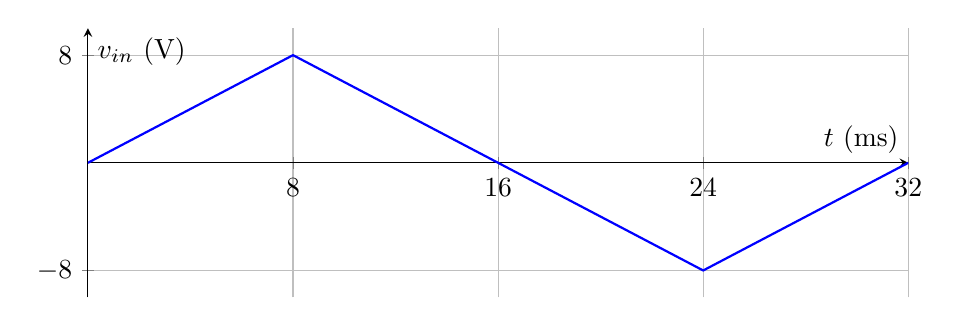
\begin{tikzpicture}
        \begin{axis}[
            width=12cm, height=5cm,
            xlabel={$t$ (ms)}, ylabel={$v_{in}$ (V)},
            xmin=0, xmax=32, ymin=-10, ymax=10,
            grid=both,
            axis lines=middle,
            xtick={0,8,16,24,32},
            ytick={-8,0,8}
        ]
        \draw[thick, blue] (0,0) -- (8,8) -- (24,-8) -- (32,0);
        \end{axis}
    \end{tikzpicture}
    \end{center}}

\begin{answer}[3.5in]
        The output is the rectified input minus the $1.0\text{V}$ dead zone.
        
        \textbf{1. Calculate Slope:}
        The wave rises from $0\text{V}$ to $8\text{V}$ in $8\text{ms}$.
        \[ \text{Slope} = \frac{8\text{V}}{8\text{ms}} = 1\text{V/ms} \]
        
        \textbf{2. Calculate Zero Crossings:}
        The output is zero when $|v_{in}| < 1.0\text{V}$.
        With a slope of $1\text{V/ms}$, the voltage reaches $1.0\text{V}$ at exactly $\mathbf{1\text{ms}}$.
        
        \textbf{3. Calculate Peak:}
        \[ v_{r(peak)} = 8\text{V} - 1.0\text{V} = \mathbf{7.0\text{V}} \]
        
        \begin{center}
        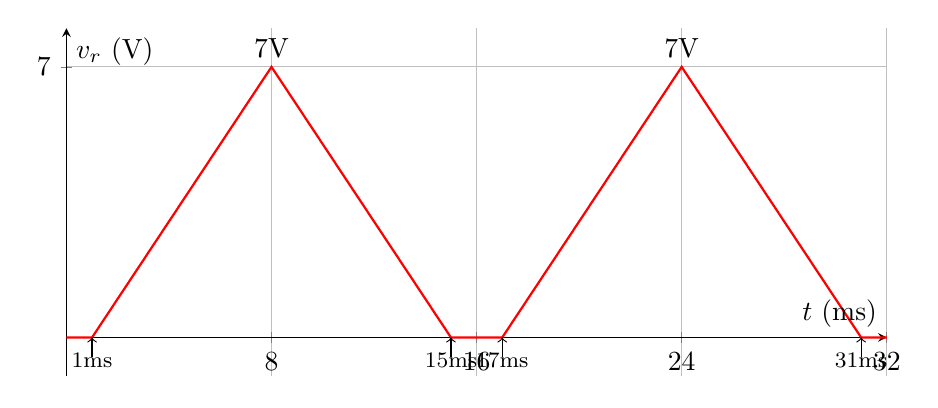
\begin{tikzpicture}
            \begin{axis}[
                width=12cm, height=6cm,
                xlabel={$t$ (ms)}, ylabel={$v_r$ (V)},
                xmin=0, xmax=32, ymin=-1, ymax=8,
                grid=both,
                axis lines=middle,
                xtick={0,8,16,24,32},
                ytick={0, 7}
            ]
            % Slope is 1V/ms.
            % Pulse 1 (Positive): Starts at 1ms, Peak at 8ms, Ends at 15ms.
            % Pulse 2 (Negative Rectified): Starts at 17ms, Peak at 24ms, Ends at 31ms.
            
            \draw[thick, red] (0,0) -- (1,0) -- (8,7) -- (15,0) -- (17,0) -- (24,7) -- (31,0) -- (32,0);
            
            % Peak Labels
            \node[anchor=south] at (8,7) {7V};
            \node[anchor=south] at (24,7) {7V};
            
            % Dead Zone Labels
            \draw[->, black] (1, -0.5) -- (1, 0) node[pos=-0.2] {\footnotesize 1ms};
            \draw[->, black] (15, -0.5) -- (15, 0) node[pos=-0.2] {\footnotesize 15ms};
            \draw[->, black] (17, -0.5) -- (17, 0) node[pos=-0.2] {\footnotesize 17ms};
            \draw[->, black] (31, -0.5) -- (31, 0) node[pos=-0.2] {\footnotesize 31ms};
            
            \end{axis}
        \end{tikzpicture}
        \end{center}
\end{answer}

\end{partquestion}

\end{mainquestion}
